%\usepackage{graphicx}

\section{Project description}
The purpose with the project work is to construct a Pan and Tilt system, for the  shown in figure \ref{fig:pantilysystem}, so that it is possible to control the system from one or more user inputs eg a joystick, a keyboard, buttons or via commands from a computer. In addition shall the system also give the user options for feedback of significant system parameters.

\begin{figure}[htb]
	\begin{center}
	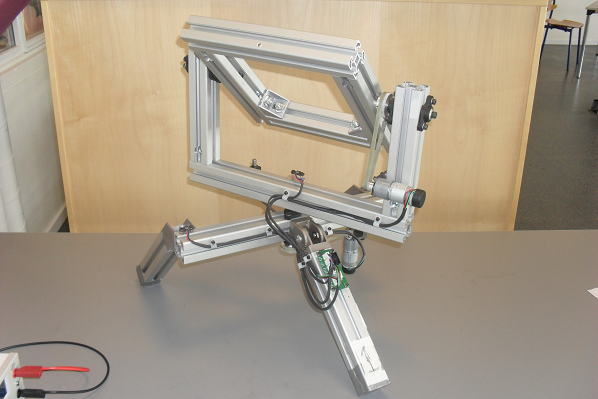
\includegraphics[scale=1,trim=0 0 0 0]{graphics/pantiltsystem.png} %trim=l b r t (can cut off from every side)
	\caption{The given pant tilt system.}
	\label{fig:pantilysystem}			% figure labels are of the form \label{fig:*}
	\end{center}
\end{figure}

\begin{itemize}
\item A system analysis and modulation of the systems individual elements.
\item Analysis and design of the regulation loops in Matlab and Simulink.
\item Documentation of FPGA design and implementation.
\item Documentation of the microprocessor programs design and implementation, including division into tasks and selection of scheduling.
\item Test and verification of the system.
\end{itemize}

It is up to the project group to chose the regulator system og the regulator loops' characteristics.

\section{Requirements}

The following conditions are set for the system:
\begin{itemize}
\item The regulators' must be implemented on a microprocessor.
\item SPI must be used in communication between the microprocessor and the FPGA.
\item The FPGA shall control the PWM signals to the motors.
\item The FPGA shall be used to determine the motors position via the encoders.
\end{itemize}

\section{The physical system}

The following is provided for the project:

\begin{itemize}
\item 2 pc. Pan and Tilt setup, that is to be shared between the project groups.
\item Motor with built in encoder to every project group.
\item Print with double H-bridge to every project group.
\end{itemize}

For the rest of the system the following devices are used:

\begin{itemize}
\item The microprocessor is a Stellaris LM3S6965 on an Evaluation Board, which is mounted on a test board with keypad, incremental rotary encoder, potentiometer and an LCD.
\item All hardware for user interface is from the given ARM test board.
\item The FPGA is a Xilinx Nexys 2 board with a Spartan-3E chip on board.
\item The SPI connection is made by connecting wires between ports on the to boards.
\end{itemize}

The pysical system was set up as following as shown in figure \ref{fig:digitalsystem}. All the user interface mounted with the microprocessor, all the motor input and output at the FPGA and a SPI connection between the two:

\begin{figure}[htb]
	\begin{center}
	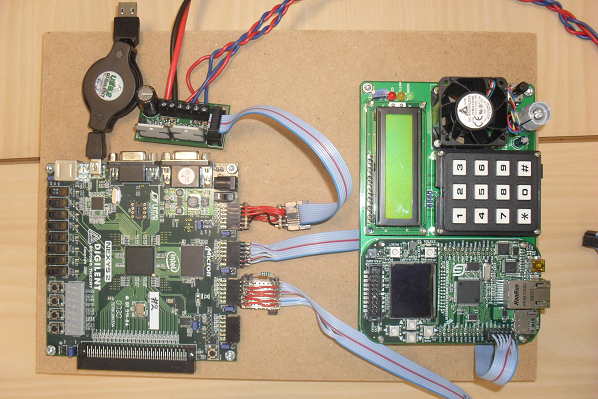
\includegraphics[scale=1,trim=0 0 0 0]{graphics/digitalsystem.png} %trim=l b r t (can cut off from every side)
	\caption{Setup of the electrical system.}
	\label{fig:digitalsystem}			% figure labels are of the form \label{fig:*}
	\end{center}
\end{figure}

\section{Complete system}

The complete system is shown in figure \ref{fig:completesystem}, here are all individual components that need to be created for the system. The exact number of tasks is not meant to be shown, but as a reference to understand the analysis of the system.

(Diagrammet skal aendres!)

Meningen er at der skal være en lille analyse af hvad der skal udvikles/ hvordan systemet skal se ud...


\begin{figure}[htb]
	\begin{center}
	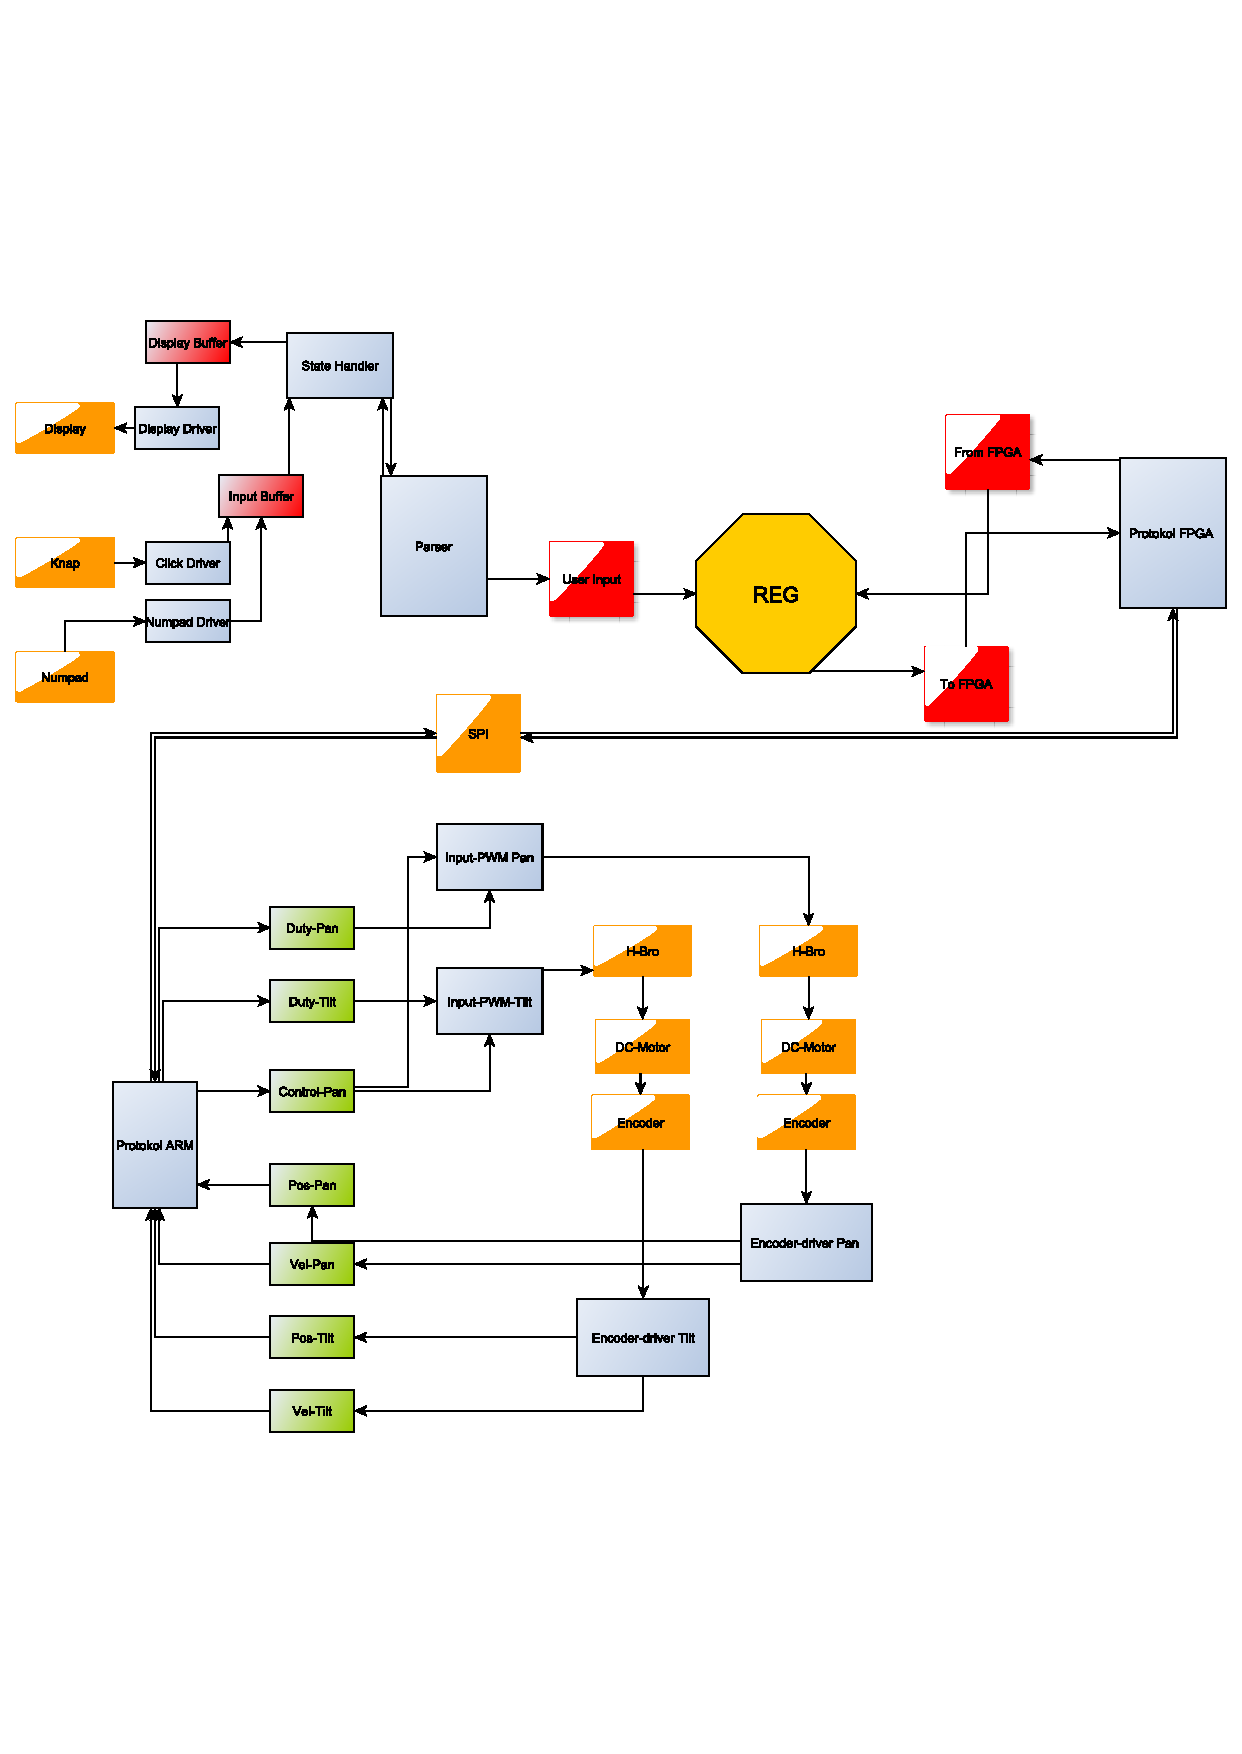
\includegraphics[scale=0.8,trim=100 130 100 250]{graphics/Project4GreaterPresentation3.pdf} %trim=l b r t (can cut off from every side)
	\caption{Setup of the complete system. Orange are physical components. Red are variables. Blue are tasks. Green are RAM. }
	\label{fig:completesystem}			% figure labels are of the form \label{fig:*}
	\end{center}
\end{figure}